\def\pgfsysdriver{pgfsys-dvisvgm.def}
% flashcards-title: Spread and compact arrangements of the same material
% flashcards-desc: A broad thin sheet and a compact rolled form are shown with identical material marks and separate text labels.
\documentclass[tikz,border=6pt]{standalone}
\usetikzlibrary{arrows.meta,calc,fit,positioning,shapes.geometric}

\definecolor{fcink}{HTML}{17212B}
\definecolor{fcblue}{HTML}{1D5D8C}
\definecolor{fcgreen}{HTML}{2D6A4F}
\definecolor{fcorange}{HTML}{A44A1F}
\definecolor{fcpale}{HTML}{F4F7F9}
\definecolor{fcsoil}{HTML}{8B5E3C}

\tikzset{
  fc text/.style={font=\sffamily, text=fcink},
  fc panel/.style={draw=fcink, line width=0.9pt, rounded corners=5pt, fill=fcpale},
  fc node/.style={draw=fcink, line width=0.9pt, rounded corners=4pt, fill=white,
    minimum width=24mm, minimum height=10mm, align=center, font=\sffamily},
  fc arrow/.style={-{Stealth[length=3.2mm,width=2.4mm]}, line width=1.2pt,
    draw=fcblue, line cap=butt},
  fc boundary/.style={draw=fcorange, line width=1.4pt, dash pattern=on 5pt off 3pt,
    rounded corners=7pt},
  fc label/.style={font=\sffamily\bfseries, text=fcink},
  fc note/.style={font=\sffamily\small, text=fcink, align=center}
}

\begin{document}
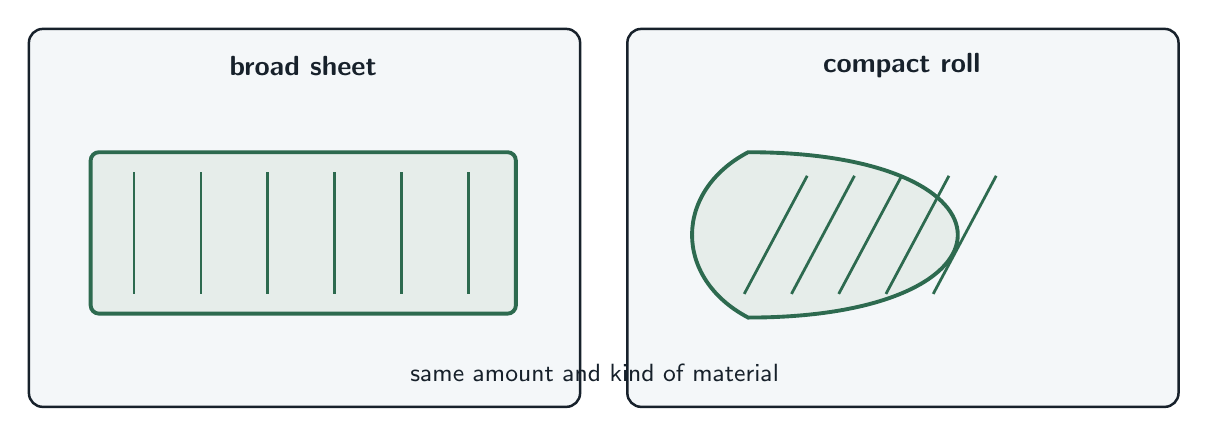
\begin{tikzpicture}[fc text, x=1cm, y=1cm]
  \node[fc panel, minimum width=70mm, minimum height=48mm, anchor=south west] at (0,0) {};
  \node[fc panel, minimum width=70mm, minimum height=48mm, anchor=south west] at (7.6,0) {};
  \node[fc label] at (3.5,4.35) {broad sheet};
  \node[fc label] at (11.1,4.35) {compact roll};
  \draw[draw=fcgreen, fill=fcgreen!12, line width=1.4pt, rounded corners=3pt]
    (0.8,1.2) rectangle (6.2,3.25);
  \foreach \x in {1.35,2.2,3.05,3.9,4.75,5.6} {\draw[draw=fcgreen, line width=1pt] (\x,1.45)--(\x,3.0);}
  \draw[draw=fcgreen, fill=fcgreen!12, line width=1.4pt]
    (9.15,1.15) .. controls (12.7,1.15) and (12.7,3.25) .. (9.15,3.25)
    .. controls (8.2,2.75) and (8.2,1.65) .. cycle;
  \foreach \x in {9.1,9.7,10.3,10.9,11.5} {\draw[draw=fcgreen, line width=1pt] (\x,1.45)--(\x+0.8,2.95);}
  \node[fc note] at (7.2,0.45) {same amount and kind of material};
\end{tikzpicture}
\end{document}
